\documentclass[journal]{IEEEtran}

\usepackage[T1]{fontenc}
\usepackage{cite}
\usepackage{amsmath,amssymb}
\usepackage{graphicx}
\usepackage{booktabs}
\usepackage{array}
\usepackage{url}
\usepackage{tikz}
\usetikzlibrary{positioning,arrows.meta,shapes.geometric}
\renewcommand{\ttdefault}{lmtt}

\hyphenation{Omni-Doc-Bench Unlimited-OCR Deep-Seek}

\begin{document}

\title{Running Unlimited-OCR on a 16\,GB Laptop:\\ Reproduction, Failure Analysis and\\ Inference-Time Repairs on OmniDocBench}

\author{Akhilesh~Reddy,~Vedansh~Saini,~and~Yug~Khatri%
\thanks{The authors are with the Indian Institute of Technology (BHU),
Varanasi, India. Roll numbers: A.~Reddy 23155018, V.~Saini 23218010,
Y.~Khatri 23155127.}%
\thanks{Project report submitted November 2026.}}

\markboth{Project Report, November~2026}%
{Reddy \MakeLowercase{\textit{et al.}}: Running Unlimited-OCR on a 16\,GB Laptop}

\maketitle

\begin{abstract}
Unlimited-OCR is an end-to-end document parser that reads page images into
Markdown and reports state-of-the-art accuracy on OmniDocBench v1.6. Its
Reference Sliding Window Attention (R-SWA) keeps the decoder's key-value cache at
a fixed size, so memory does not grow with output length. The official release
targets NVIDIA GPUs only. We run the released weights, unchanged, on a 16\,GB
Apple Silicon laptop through the MLX framework under a 7.5\,GB memory cap, and
ask two questions: does the published accuracy hold on this hardware, and can
inference-time changes fix the cases where it does not? On a stratified
140-page sample, our setup matches the paper within bootstrap intervals (text
edit distance 0.036 against 0.042, table TEDS 92.4 against 90.2). On the full
1,651-page benchmark it reaches an Overall score of 90.08 against the reported
93.92; formula recognition (CDM 87.10 against 95.79) accounts for 2.90 of the
3.84-point gap. The text error is concentrated: 36 pages carry 37\% of it,
mostly repetition loops that the model's own n-gram guard cannot see. A ladder
of inference-time repairs (a coordinate- and number-blind loop guard, a
low-resolution fallback with a guard for dense pages, and output clean-up)
lowers text edit distance on the 50 worst pages from 0.685 to 0.427 and raises
table TEDS from 29.3 to 45.2, with no regression on a separate development set.
We also report two repairs that helped every subset yet cost 3.6 TEDS on the
full benchmark, and were rejected.
\end{abstract}

\begin{IEEEkeywords}
Document parsing, optical character recognition, OmniDocBench, reproducibility,
sliding window attention, mixture of experts, Apple Silicon, MLX.
\end{IEEEkeywords}

\IEEEpeerreviewmaketitle

% =====================================================================
\section{Introduction}

\IEEEPARstart{E}{nd-to-end} OCR models replace the classic pipeline of layout
detection, text recognition and reading-order recovery with a single
vision-language model that writes a page out as structured text
\cite{blecher2023nougat,wei2024got,wei2025deepseekocr}. Their decoder keeps a
key-value (KV) cache that grows with every output token, so long documents
become slower and need more memory as decoding goes on.

Unlimited-OCR \cite{baidu2026unlimited} addresses this with Reference Sliding
Window Attention (R-SWA): each output token attends to the whole image prefix but
only to the most recent 128 output tokens. The paper reports state-of-the-art
results on OmniDocBench v1.6 \cite{ouyang2025omnidocbench}, including an Overall
score of 93.92. The released code, however, runs only on NVIDIA GPUs, and the
model was trained on 128 A800 GPUs.

This project asks whether those results hold on commodity hardware: a 16\,GB
Apple Silicon laptop running the released weights through MLX
\cite{hannun2023mlx}. Where they do not, we look for the cause and test fixes
that need no training. Our contributions are:

\begin{enumerate}
\item A working setup on a 16\,GB laptop: two defects in a community MLX port
were found and fixed, and peak memory was brought under a 7.5\,GB cap.
\item A reproduction study. On a stratified 140-page sample, text and table
accuracy match the paper within 95\% bootstrap intervals. On all 1,651 pages,
including the formula metric CDM \cite{wang2025cdm}, we reach an Overall score of
90.08 against 93.92 and break the gap down by metric.
\item A failure analysis showing that the error is concentrated in a few dozen
pages, and why the model's built-in repetition guard misses most of its loops.
\item A set of inference-time repairs, each tested page by page against a
baseline on a problem set, a development set and the full benchmark, including
two repairs rejected on the full benchmark after passing on both subsets.
\end{enumerate}

% =====================================================================
\section{Background}

\subsection{Unlimited-OCR}

Unlimited-OCR continues training from DeepSeek-OCR \cite{wei2025deepseekocr}.
Its vision encoder (DeepEncoder) chains a SAM ViT-B \cite{kirillov2023sam} with
window attention and a CLIP-L \cite{radford2021clip} with global attention, and
compresses visual tokens 16 times, so a $1024\times1024$ page becomes 256 tokens.
A linear projector feeds a DeepSeek-V2-style \cite{deepseek2024v2}
mixture-of-experts decoder: 12 layers, 64 routed experts with 6 active per token,
2 shared experts, about 3B parameters in total and 0.5B active per token.

Two image modes exist. \emph{Gundam} mode adds $640\times640$ crops to a global
view and is used for single pages; \emph{Base} mode uses one $1024\times1024$
view per page and is used for multi-page input. Decoding is greedy, with a
guard that bans any 35-token sequence already seen in the recent output.

R-SWA is applied in every decoder layer. With a prefix of $L_m$ tokens (image and
prompt) and a window of $n=128$ output tokens, the cache after $T$ output tokens
holds
\begin{equation}
|\mathrm{KV}_T| = L_m + \min(n, T)
\end{equation}
entries instead of $L_m + T$. Unlike a plain sliding window
\cite{beltagy2020longformer}, the prefix is never dropped, so every token can
still see the whole page. The paper names its own main weakness: repetition
loops on small text in long documents.

\subsection{OmniDocBench and its metrics}

OmniDocBench v1.6 \cite{ouyang2025omnidocbench} has 1,651 annotated pages of
nine document types (slides, academic papers, books, textbooks, exam papers,
magazines, newspapers, notes and research reports) plus a few historical
documents. Its official evaluator matches predicted blocks to ground truth and
reports:

\begin{itemize}
\item \emph{Text edit distance} (lower is better): the Levenshtein distance
\cite{levenshtein1966} between matched text blocks, normalised by length,
\begin{equation}
\mathrm{NED}(p,g) = \frac{\mathrm{Lev}(p,g)}{\max(|p|,|g|)}.
\end{equation}
\item \emph{Table TEDS} \cite{zhong2020teds} (higher is better): a tree edit
distance between predicted and ground-truth table HTML,
$\mathrm{TEDS}(T_a,T_b) = 1 - \mathrm{EditDist}(T_a,T_b)/\max(|T_a|,|T_b|)$,
reported in percent. \emph{TEDS-S} ignores cell text and scores structure only.
\item \emph{Formula CDM} \cite{wang2025cdm} (higher is better): both formulas are
rendered from LaTeX and compared character by character in image space, which
avoids penalising equivalent LaTeX spellings.
\item \emph{Reading-order edit distance} (lower is better): edit distance over
the order of matched blocks.
\end{itemize}
The headline score combines the first three:
\begin{equation}
\mathrm{Overall} = \tfrac{1}{3}\bigl(100\,(1-\mathrm{NED}_{\mathrm{text}}) +
\mathrm{TEDS} + \mathrm{CDM}\bigr).
\label{eq:overall}
\end{equation}
Table~\ref{tab:paper} lists the reported results we test.

\begin{table}[!t]
\caption{Results Reported in the Unlimited-OCR Paper \cite{baidu2026unlimited}}
\label{tab:paper}
\centering
\footnotesize
\setlength{\tabcolsep}{3.2pt}
\begin{tabular}{@{}lcccccc@{}}
\toprule
Model (OmniDocBench) & Overall & Text & CDM & TEDS & TEDS-S & Order \\
\midrule
DeepSeek-OCR (v1.5) & 87.01 & 0.073 & 83.37 & 84.97 & 88.80 & 0.086 \\
Unlimited-OCR (v1.5) & 93.23 & 0.038 & 92.61 & 90.93 & 94.07 & 0.045 \\
Unlimited-OCR (v1.6) & 93.92 & 0.042 & 95.79 & 90.16 & 93.32 & 0.129 \\
\bottomrule
\end{tabular}
\end{table}

% =====================================================================
\section{Experimental Setup}

\subsection{Hardware and software}

All model runs use one MacBook Air with an Apple M5 chip (10 cores) and 16\,GB of
unified memory. The model runs through a community MLX port
(\texttt{shubhxho/Unlimited-OCR-MLX}, commit \texttt{e4c39cd}) on
\texttt{mlx-vlm} 0.6.16 \cite{canuma2024mlxvlm} and MLX 0.32.1, with the
released weights (\texttt{baidu/Unlimited-OCR}, revision \texttt{07dea83}) in
bf16 and greedy decoding. Scoring uses OmniDocBench v1.6 (dataset revision
\texttt{aa1ee96}) and the official evaluator at commit \texttt{f133a71}.

\subsection{Corrections to the MLX port}

Two defects had to be fixed before any measurement:
\begin{enumerate}
\item \emph{Decoding crash.} The port's repetition guard returned logits without
their batch dimension under \texttt{mlx-vlm} 0.6.16, so every run failed on the
first generated token. The fix restores the shape and leaves the banned-token
rule unchanged; a unit test reproduces the defect.
\item \emph{Prompt mismatch.} The port's prompt ended with a space token that
the reference code strips. This made the model skip the opening paragraph of a
page and invent a date. Removing the space fixed both and left the rest of the
output identical.
\end{enumerate}

\subsection{Memory cap}

Every run is capped at 7.5\,GB so the laptop stays usable. Meeting the cap
needed changes to how image crops are processed; peak memory fell from 10.0\,GB
to under 8\,GB.

\subsection{Formula scoring}

CDM needs a Linux \TeX{} toolchain, so it was run on a second machine in the
evaluator's own Docker image, on the 313 pages that contain display formulas
(2,352 formulas, no timeouts or errors, 1\,h\,50\,min).

\subsection{Page sets and statistics}

We use four page sets:
\begin{itemize}
\item the \emph{full benchmark} (1,651 pages, about 10 hours per model run);
\item a \emph{reproduction sample} of 140 pages (15 per document type plus all 5
historical documents, seed 42);
\item a disjoint 45-page \emph{development set} (5 per type), used to check that
a repair harms nothing;
\item a 50-page \emph{problem set} drawn from the first full run: the 36 pages
with text edit $\geq 0.5$, 17 pages with zero table TEDS, 4 pages that regressed
under the memory cap, and 2 normal controls (with overlap).
\end{itemize}
Per-type means are reweighted to the full benchmark's type mix. Intervals are
95\% stratified bootstrap intervals \cite{efron1993bootstrap} from 2,000
resamples, with pages resampled within type. A change is compared with its
baseline page by page and counts as an improvement only if the interval of the
paired difference excludes zero.

% =====================================================================
\section{Reproduction}

\subsection{Stratified sample}

Table~\ref{tab:repro} compares our setup with the paper on the 140-page sample.
Every reported value falls inside our interval: the MLX setup, with the two port
corrections, reproduces the published text and table accuracy within sampling
error. Pages took 18.1\,s on average at 75 output tokens per second, with a
peak of 10.0\,GB before the memory cap was introduced.

\begin{table}[!t]
\caption{Reproduction on a 140-Page Stratified Sample}
\label{tab:repro}
\centering
\footnotesize
\begin{tabular}{@{}lcc@{}}
\toprule
Metric & This work (MLX, M5) & Paper (GPU) \\
\midrule
Text edit $\downarrow$ & 0.036 [0.024, 0.051] & 0.042 \\
Table TEDS $\uparrow$ & 92.4 [88.1, 95.9] & 90.16 \\
Table TEDS-S $\uparrow$ & 94.9 [91.7, 97.6] & 93.32 \\
Reading order $\downarrow$ & 0.107 [0.078, 0.142] & 0.129 \\
\bottomrule
\end{tabular}
\end{table}

\subsection{Full benchmark}

The first full run (E-028) covered all 1,651 pages under the memory cap.
Table~\ref{tab:full} shows it alongside the run with our kept output fixes
(E-053, Section~\ref{sec:full}). The full run is behind the paper on every
metric. The 140-page sample was too small to show this, because the shortfall
sits in a tail of rare failures:

\begin{itemize}
\item 36 pages score a text edit distance of 0.5 or worse and carry 37\% of the
total text error. Most are repetition loops that run into the 32,768-token
output limit, or broadsheet newspapers that are cut short.
\item On 137 pages run both with and without the cap, the capped run was 0.014
worse in text edit distance; four fragile pages tipped into failure.
\end{itemize}

\begin{table}[!t]
\caption{Full Benchmark (1,651 Pages). Overall Follows (\ref{eq:overall})}
\label{tab:full}
\centering
\footnotesize
\setlength{\tabcolsep}{4pt}
\begin{tabular}{@{}lccccc@{}}
\toprule
Run & Text $\downarrow$ & CDM $\uparrow$ & TEDS $\uparrow$ & Order $\downarrow$ & Overall $\uparrow$ \\
\midrule
Paper & 0.042 & 95.79 & 90.16 & 0.129 & 93.92 \\
E-028 (first run) & 0.0500 & 87.10 & 87.82 & 0.1366 & 89.97 \\
E-053 (kept fixes) & 0.0494 & 87.10 & 88.09 & 0.1355 & 90.08 \\
\bottomrule
\end{tabular}
\end{table}

\subsection{Where the Overall gap comes from}

Because (\ref{eq:overall}) is a plain mean, the 3.84-point gap between E-053 and
the paper splits exactly by metric (Fig.~\ref{fig:gap}). Formulas account for
2.90 points, tables for 0.69 and text for 0.25. Pooled over all formulas rather
than averaged per page, CDM is 90.07. The repairs in Section~\ref{sec:repairs}
do not change formula output, so the same CDM applies to E-028 and E-053.

\begin{figure}[!t]
\centering
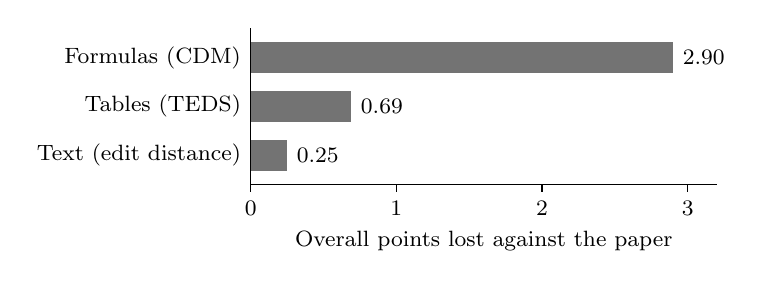
\begin{tikzpicture}[x=1.85cm,y=0.62cm,font=\footnotesize]
  \foreach \v/\lab/\y in {2.90/Formulas (CDM)/2, 0.69/Tables (TEDS)/1, 0.25/Text (edit distance)/0}{
    \fill[black!55] (0,\y-0.32) rectangle (\v,\y+0.32);
    \node[left] at (0,\y) {\lab};
    \node[right] at (\v,\y) {\v};
  }
  \draw (0,-0.6) -- (0,2.6);
  \draw (0,-0.6) -- (3.2,-0.6);
  \foreach \t in {0,1,2,3}{\draw (\t,-0.6) -- (\t,-0.75) node[below] {\t};}
  \node[below] at (1.6,-1.35) {Overall points lost against the paper};
\end{tikzpicture}
\caption{Breakdown of the 3.84-point Overall gap between E-053 (90.08) and the
paper (93.92). Formula recognition is the largest part.}
\label{fig:gap}
\end{figure}

% =====================================================================
\section{Inference-Time Repairs}
\label{sec:repairs}

Training is out of reach on a laptop, so every change works at inference time on
the released weights. Fig.~\ref{fig:pipeline} shows where each one sits, and
Table~\ref{tab:changes} lists every change we tested.

\begin{figure}[!t]
\centering
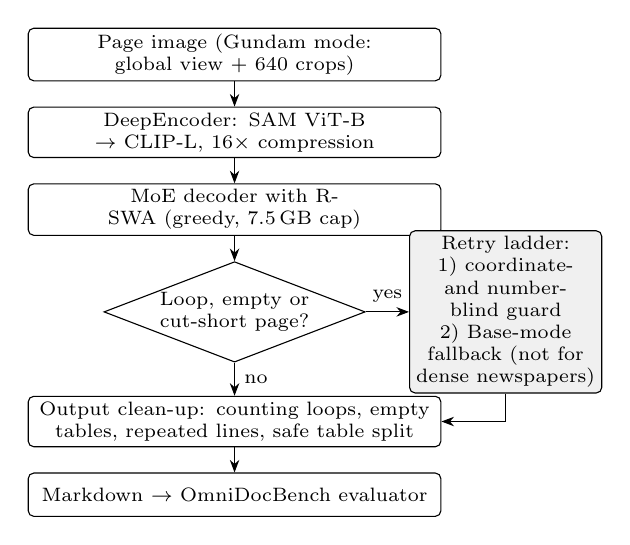
\begin{tikzpicture}[
  font=\scriptsize,
  box/.style={draw, rounded corners=2pt, align=center, text width=5.1cm, minimum height=0.55cm, inner sep=2pt},
  side/.style={draw, rounded corners=2pt, align=center, text width=2.3cm, inner sep=2pt, fill=black!6},
  dec/.style={draw, diamond, aspect=2.6, align=center, inner sep=0.5pt},
  arr/.style={-{Stealth[length=1.6mm]}},
  node distance=0.32cm]
  \node[box] (img) {Page image (Gundam mode: global view + 640 crops)};
  \node[box, below=of img] (enc) {DeepEncoder: SAM ViT-B $\rightarrow$ CLIP-L, 16$\times$ compression};
  \node[box, below=of enc] (dec) {MoE decoder with R-SWA (greedy, 7.5\,GB cap)};
  \node[dec, below=of dec] (flag) {Loop, empty or\\ cut-short page?};
  \node[box, below=0.42cm of flag] (post) {Output clean-up: counting loops, empty tables, repeated lines, safe table split};
  \node[box, below=of post] (md) {Markdown $\rightarrow$ OmniDocBench evaluator};
  \node[side, right=0.55cm of flag] (retry) {Retry ladder:\\ 1) coordinate- and number-blind guard\\ 2) Base-mode fallback (not for dense newspapers)};
  \draw[arr] (img) -- (enc);
  \draw[arr] (enc) -- (dec);
  \draw[arr] (dec) -- (flag);
  \draw[arr] (flag) -- node[right] {no} (post);
  \draw[arr] (flag) -- node[above] {yes} (retry);
  \draw[arr] (retry.south) |- (post.east);
  \draw[arr] (post) -- (md);
\end{tikzpicture}
\caption{Inference pipeline. Shaded: the retry ladder, which runs only on flagged
pages. All other pages keep their first decode.}
\label{fig:pipeline}
\end{figure}

\begin{table*}[!t]
\caption{Inference-Time Changes Tested}
\label{tab:changes}
\centering
\footnotesize
\begin{tabular}{@{}p{3.9cm}p{8.7cm}p{4.2cm}@{}}
\toprule
Change & What it does & Outcome \\
\midrule
Coordinate-blind loop guard & Re-decodes looping pages with the 35-token guard applied to text with box markers removed. & Kept \\
Number-blind loop guard & Also blocks loops that change only a number each time (``(1) item'', ``(2) item'', \dots). & Kept: largest single gain \\
Base-mode fallback & Re-reads pages that come back empty or cut short in Gundam mode using Base mode. & Kept \\
Fallback guard & Keeps dense newspapers out of Base mode, which blurs them. & Kept \\
Output clean-up & Cuts counting loops, runaway empty tables and repeated lines. & Kept \\
Safe table splitter & Splits stacked tables only when the column count changes or a row repeats the header. & Kept: +0.26 TEDS on full set \\
Page-by-page long documents & Decodes a long document one page per request and joins the outputs. & Kept \\
8-bit weights, bf16 fallback & Quantised decoder; flagged pages are re-run in bf16. & Kept as a speed option \\
4 routed experts instead of 6 & Less work per token. & Kept as a speed option \\
4-bit weights & Smaller, faster decoder. & Rejected: loses tables \\
First table splitter, prose unwrapping & Split tables at any break; turn one-row tables into text. & Rejected: $-3.6$ TEDS on full set \\
Drop headers and page numbers & Removes page furniture from the output. & Rejected: slightly worse \\
Best of two decodes & Keeps the more confident of two readings. & Rejected: no gain \\
\bottomrule
\end{tabular}
\end{table*}

\subsection{Why the built-in guard misses loops}

When the model loops, it opens a new layout block for each repeat, and each
block starts with fresh box coordinates of the form
\texttt{<|det|>type [x1,y1,x2,y2]<|/det|>}. Because the coordinates change, no 35
consecutive tokens repeat exactly, and the decode-time guard never fires. On one
development page the model repeated a single sentence 555 times until it hit the
output limit.

We flag a page when the text of one block, with its marker removed, repeats six
or more times, or when a marker is left unclosed. The threshold was fixed before
looking at test pages. Flagged pages are re-decoded with the same 35-token rule
applied to the text with marker spans removed. A second version also replaces
digits before comparing, which catches numbered loops such as ``(1) item'',
``(2) item''. On the development page above, repair cut the page's text edit
distance from 0.829 to 0.371 and its decode time by 95\%.

\subsection{Resolution fallback and its guard}

Some pages come back empty or stop early in Gundam mode. These are re-read in
Base mode, which uses a single global view. Base mode blurs dense broadsheet
newspapers, so a guard keeps those pages out of the fallback. The guard was
added after an earlier version sent an exam page to the wrong mode and took its
text edit distance from 0.008 to 0.936.

\subsection{Output clean-up}

Three rules act on the decoded text: they cut counting loops, runaway empty
tables and repeated lines. A fourth splits tables that the model has merged. Its
first version split at any full-width row; the kept version splits only when the
column count changes or a row repeats the header's words.

% =====================================================================
\section{Results}

\subsection{Problem set}

Table~\ref{tab:ladder} shows each repair added in turn on the 50-page problem
set. With only the kept repairs (E-055), text edit distance fell by 0.258
[0.107, 0.412] to 0.427, reading-order distance fell by 0.198 [0.080, 0.317], and
table TEDS rose by 15.9 [4.3, 30.1] to 45.2. E-049 reached a lower 0.397 by also
using prose unwrapping and the first table splitter, which were rejected on the
full benchmark. The problem set was chosen from the worst pages, so these gains
measure how much is repaired, not a benchmark score.

\begin{table}[!t]
\caption{Repair Ladder on the 50-Page Problem Set}
\label{tab:ladder}
\centering
\footnotesize
\setlength{\tabcolsep}{4pt}
\begin{tabular}{@{}lcc@{}}
\toprule
Step & Text edit $\downarrow$ & TEDS $\uparrow$ \\
\midrule
Baseline (E-030) & 0.685 & 29.3 \\
+ number-blind loop guard (E-039) & 0.564 & 30.6 \\
+ Base fallback, empty pages (E-043) & 0.500 & 30.6 \\
+ table split, repeated lines (E-044) & 0.500 & 35.4 \\
+ Base fallback, cut-short pages (E-046) & 0.438 & 40.3 \\
+ prose-table unwrapping (E-047) & 0.408 & 40.3 \\
+ fallback guard (E-049) & 0.397 & 45.3 \\
\midrule
Kept repairs only, safe splitter (E-055) & 0.427 & 45.2 \\
\bottomrule
\end{tabular}
\end{table}

\subsection{Development set}

On the 45-page development set the same repairs changed one page, which
improved (text edit 0.055 to 0.054). No page became worse. The safe table
splitter changed no development page.

\subsection{Full benchmark}
\label{sec:full}

Two repairs that helped both the problem set and the development set failed on
the full benchmark. The first table splitter broke valid tables at full-width
section headers (33 pages worse, 6 better), and prose unwrapping turned valid
one-row tables into text (6 worse, none better). Together they cost 3.6 TEDS
(87.82 to 84.20; E-051) and were rejected.

The kept clean-up rules and the safe splitter, applied to all 1,651 pages
without a new model run (E-053), give text edit 0.0494 [0.0435, 0.0558],
reading order 0.1355 [0.1256, 0.1458], TEDS 88.09 [85.58, 90.31] and TEDS-S
91.74 [89.70, 93.54]. Paired against E-028, text edit improved by 0.0006
[0.0000, 0.0016], reading order by 0.0010 [0.0002, 0.0021] and TEDS by 0.26
[0.01, 0.64], with no table made worse. The retry ladder, which needs new model
runs, has not yet been applied to the full benchmark: 52 pages are flagged, 23
of which already have problem-set output.

\subsection{Long documents}

The paper's long-document set is not public, so we use 2- to 40-page prefixes
of three public NIST reports scored against the PDF text layer. Absolute values
are therefore not comparable with the paper; Table~\ref{tab:long} compares
methods on the same documents.

\begin{table}[!t]
\caption{Long Documents: One Request Against Page by Page (Base Mode)}
\label{tab:long}
\centering
\footnotesize
\setlength{\tabcolsep}{3.5pt}
\begin{tabular}{@{}ccccccc@{}}
\toprule
 & \multicolumn{3}{c}{One request} & \multicolumn{3}{c}{Page by page} \\
\cmidrule(lr){2-4}\cmidrule(l){5-7}
Pages & Edit & Recall & Time (s) & Edit & Recall & Time (s) \\
\midrule
2 & 0.138 & 0.934 & 9 & 0.136 & 0.938 & 7 \\
5 & 0.104 & 0.973 & 31 & 0.039 & 0.973 & 25 \\
10 & 0.200 & 0.959 & 86 & 0.101 & 0.958 & 64 \\
20 & 0.110 & 0.953 & 194 & 0.104 & 0.961 & 141 \\
40 & 0.228 & 0.917 & 502 & 0.077 & 0.968 & 283 \\
\bottomrule
\end{tabular}
\end{table}

R-SWA does keep memory flat: peak memory stayed between 8 and 11.4\,GB up to 40
pages in one request. In one request, however, the model added or dropped a page
in 10 of 15 documents, and two of three 40-page documents hit the output limit.
Reading one page per request removes both failures, raises recall at 40 pages
from 0.917 to 0.968 and cuts model time by 44\%.

\subsection{Speed}

Quantising the decoder to 8 bits raised output speed from about 90 to 143
tokens per second. Its one failure on the development set was a page that
looped; the loop detector caught it and a bf16 re-run restored it. With that
fallback, 8-bit weights matched bf16 accuracy (paired text edit difference
$-0.001$ [$-0.002$, 0.000]) in a third less time. 4-bit weights lost
10.3 TEDS on pages that do not loop, which no detector can route to a fallback,
so they were rejected.

% =====================================================================
\section{Discussion}

\subsection{Why the full benchmark falls short of the paper}

Our setup differs from the paper's in ways that each could cost accuracy, and
we cannot yet separate them:

\begin{itemize}
\item \emph{Runtime.} We use a community MLX port, not the official CUDA code.
Beyond the two defects we fixed, it has not been checked against the official
model output, so part of the gap may come from the port rather than the model.
\item \emph{Memory cap.} The cap costs a little accuracy on fragile pages
(+0.014 text edit on 137 matched pages).
\item \emph{Formula scoring.} The evaluator's Docker image, which computes CDM,
contains different code from the evaluator we use locally. On the same output it
reports a formula edit distance of 0.188, against 0.110 from the local evaluator.
The two match formulas to ground truth differently, so part of the formula gap
may come from matching rather than recognition.
\item \emph{Sample size.} The 140-page sample matched the paper, but the
full-set shortfall sits in rare failures that a sample of that size seldom
contains.
\end{itemize}

A decisive test is to run the official code on a CUDA GPU over the same 1,651
pages and score it with the same evaluator. If it reaches about 93.9, the paper
holds and the remaining gap belongs to the port and the memory cap.

\subsection{Lessons}

Repairs that pass on a problem set and a development set can still fail on the
full benchmark: the first table splitter and prose unwrapping looked safe on 95
pages and cost 3.6 TEDS on 1,651. Every repair is now checked on the full
benchmark before it is kept. The problem set was chosen from the worst pages,
so repairs could fit those pages too closely; the development set and the full
benchmark guard against that. Some failures cannot be repaired at inference
time: on warped scans of vertical classical Chinese, loop repair stops the loop
but cannot make the text right.

% =====================================================================
\section{Future Work}

\begin{enumerate}
\item \emph{Full-benchmark retry.} Run the retry ladder on the 29 flagged pages
that have no problem-set output yet (about 47 minutes) and rescore all 1,651
pages.
\item \emph{Formulas.} As the largest part of the gap, inspect the
lowest-scoring formula pages to see whether formulas are missed, mis-written or
mis-matched, and score them with both evaluators.
\item \emph{Reference run.} Run the official code on a CUDA GPU to separate the
port and the memory cap from the model itself.
\item \emph{Column slicing.} Split broadsheet newspapers into columns before
decoding and stitch the output back together, since the model reads very large
pages at too low a resolution.
\item \emph{Resolution routing.} Send pages with small print to high resolution
before decoding, instead of repairing them afterwards.
\end{enumerate}

% =====================================================================
\section{Conclusion}

The released Unlimited-OCR weights run on a 16\,GB laptop, and on a stratified
sample they reproduce the paper's text and table accuracy. On the full
benchmark, under an 8\,GB memory cap and a community port, they reach an Overall
score of 90.08 against the reported 93.92, and most of that gap is formula
recognition. The text error left is concentrated in a few dozen pages, largely
repetition loops that the model's own guard cannot see. Inference-time repairs
that ignore box coordinates and numbers, fall back to a lower resolution with a
guard, and clean up the output, recover a large share of the error on those
pages without harming normal ones. Testing each repair on the full benchmark,
not only on subsets, was necessary: two repairs that passed every smaller test
were rejected there.

\section*{Acknowledgment}

The authors thank the Unlimited-OCR authors for releasing their weights, the
OmniDocBench maintainers for the benchmark and evaluator, and the author of the
MLX port on which this work builds.

\begin{thebibliography}{99}

\bibitem{baidu2026unlimited}
Baidu Inc., ``Unlimited OCR works,'' \emph{arXiv preprint arXiv:2606.23050},
2026. [Online]. Available: \url{https://github.com/baidu/Unlimited-OCR}

\bibitem{wei2025deepseekocr}
H.~Wei, Y.~Sun, and Y.~Li, ``DeepSeek-OCR: Contexts optical compression,''
\emph{arXiv preprint arXiv:2510.18234}, 2025.

\bibitem{blecher2023nougat}
L.~Blecher, G.~Cucurull, T.~Scialom, and R.~Stojnic, ``Nougat: Neural optical
understanding for academic documents,'' \emph{arXiv preprint arXiv:2308.13418},
2023.

\bibitem{wei2024got}
H.~Wei \emph{et~al.}, ``General OCR theory: Towards OCR-2.0 via a unified
end-to-end model,'' \emph{arXiv preprint arXiv:2409.01704}, 2024.

\bibitem{ouyang2025omnidocbench}
L.~Ouyang \emph{et~al.}, ``OmniDocBench: Benchmarking diverse PDF document
parsing with comprehensive annotations,'' in \emph{Proc. IEEE/CVF Conf. Comput.
Vis. Pattern Recognit. (CVPR)}, 2025.

\bibitem{hannun2023mlx}
A.~Hannun, J.~Digani, A.~Katharopoulos, and R.~Collobert, ``MLX: Efficient and
flexible machine learning on Apple silicon,'' 2023. [Online]. Available:
\url{https://github.com/ml-explore/mlx}

\bibitem{canuma2024mlxvlm}
P.~Canuma, ``MLX-VLM: Vision language models on Apple silicon with MLX,'' 2024.
[Online]. Available: \url{https://github.com/Blaizzy/mlx-vlm}

\bibitem{wang2025cdm}
B.~Wang \emph{et~al.}, ``Image over text: Transforming formula recognition
evaluation with character detection matching,'' in \emph{Proc. IEEE/CVF Conf.
Comput. Vis. Pattern Recognit. (CVPR)}, 2025.

\bibitem{kirillov2023sam}
A.~Kirillov \emph{et~al.}, ``Segment anything,'' in \emph{Proc. IEEE/CVF Int.
Conf. Comput. Vis. (ICCV)}, 2023, pp. 4015--4026.

\bibitem{radford2021clip}
A.~Radford \emph{et~al.}, ``Learning transferable visual models from natural
language supervision,'' in \emph{Proc. Int. Conf. Mach. Learn. (ICML)}, 2021,
pp. 8748--8763.

\bibitem{deepseek2024v2}
DeepSeek, ``DeepSeek-V2: A strong, economical, and efficient
mixture-of-experts language model,'' \emph{arXiv preprint arXiv:2405.04434},
2024.

\bibitem{beltagy2020longformer}
I.~Beltagy, M.~E. Peters, and A.~Cohan, ``Longformer: The long-document
transformer,'' \emph{arXiv preprint arXiv:2004.05150}, 2020.

\bibitem{levenshtein1966}
V.~I. Levenshtein, ``Binary codes capable of correcting deletions, insertions,
and reversals,'' \emph{Soviet Physics Doklady}, vol.~10, no.~8, pp. 707--710,
1966.

\bibitem{zhong2020teds}
X.~Zhong, E.~ShafieiBavani, and A.~Jimeno~Yepes, ``Image-based table
recognition: Data, model, and evaluation,'' in \emph{Proc. Eur. Conf. Comput.
Vis. (ECCV)}, 2020, pp. 564--580.

\bibitem{efron1993bootstrap}
B.~Efron and R.~J. Tibshirani, \emph{An Introduction to the Bootstrap}.
\hskip 1em plus 0.5em minus 0.4em\relax New York, NY, USA: Chapman \& Hall,
1993.

\end{thebibliography}

\end{document}
